
\section{Stehwellenverhältnis (SWR)}
\label{section:swr}
\begin{frame}%STARTCONTENT
\begin{itemize}
  \item Passt der Speisewiderstand der Antenne nicht zum Wellenwiderstand der Zuleitung, kommt es zu einer \emph{Reflexion}
  \item Sendeleistung wird zum Funkgerät zurück reflektiert $\rightarrow$ kann nicht an der Antenne abgestrahlt werden
  \item Stimmen Speisewiderstand der Antenne und Wellenwiderstand der Speiseleitung überein, liegt \emph{Anpassung} vor
  \end{itemize}
\end{frame}

\begin{frame}
\frametitle{SWR-Meter}
Misst gleichzeitig die Sendeleistung zur Antenne und die reflektierte, rücklaufende Leistung
\begin{columns}
    \begin{column}{0.48\textwidth}
    
\begin{figure}
    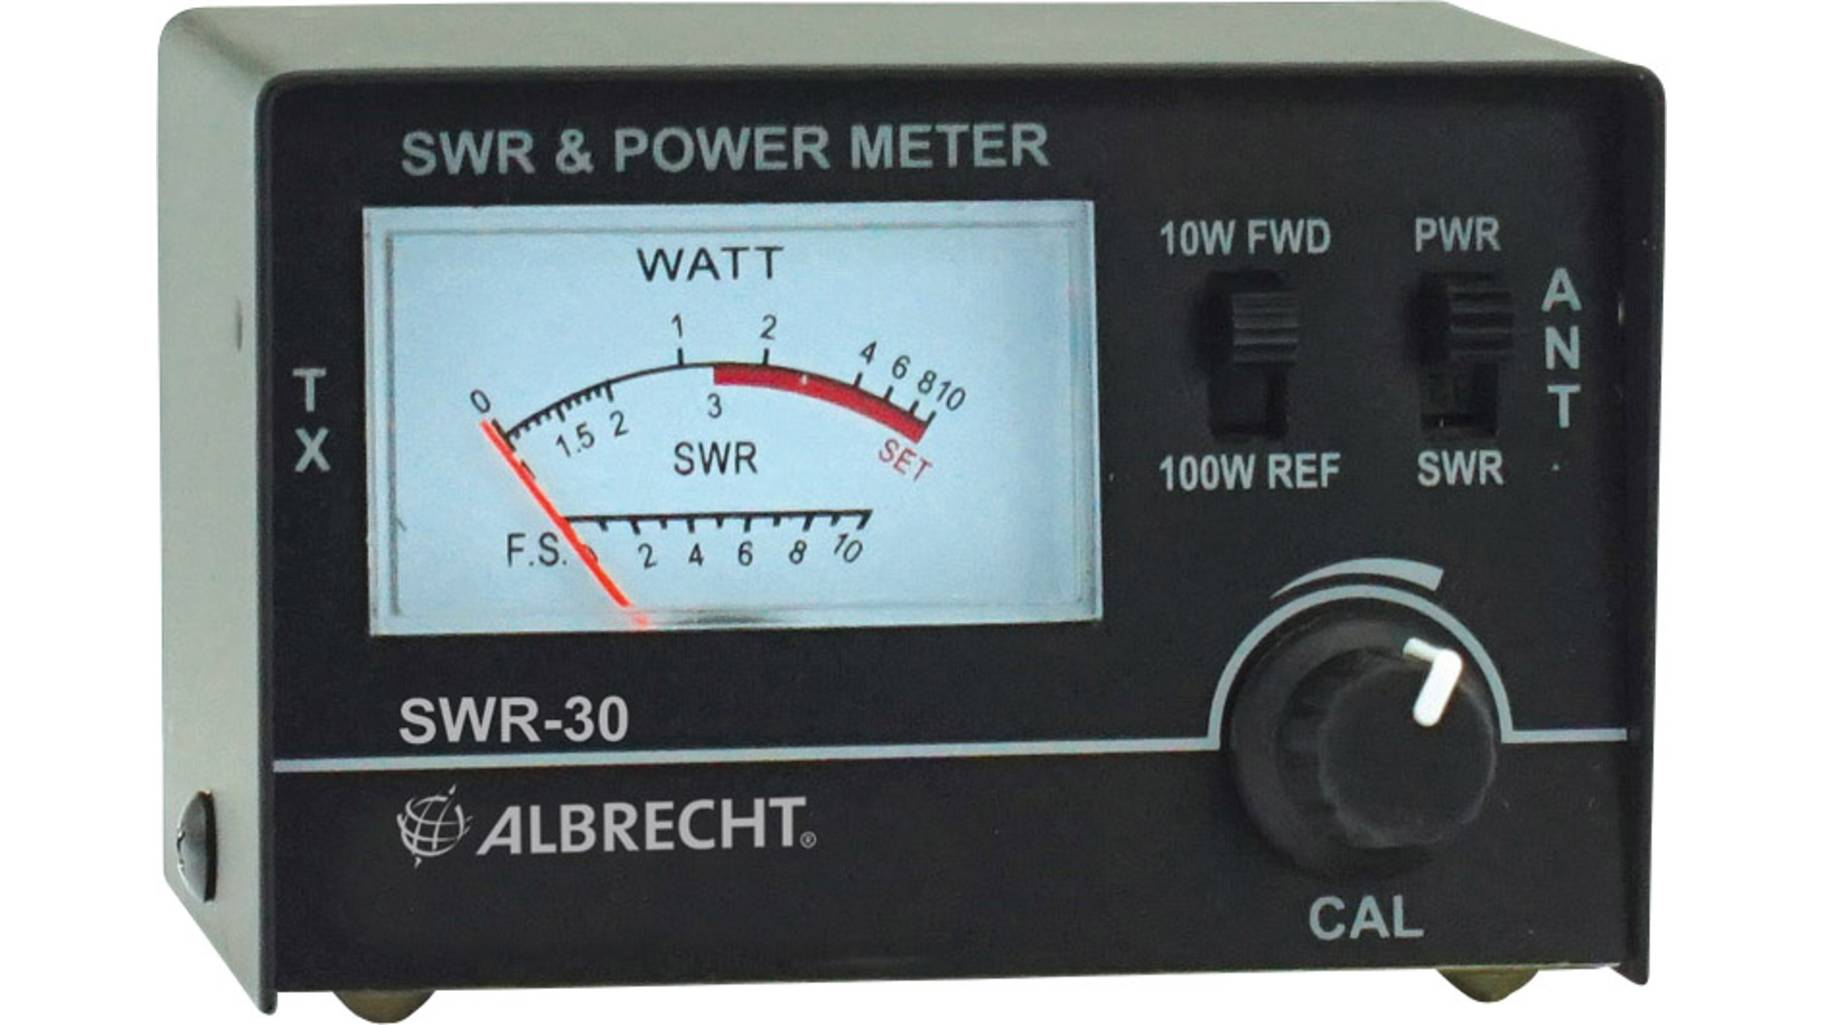
\includegraphics[width=0.85\textwidth]{foto/144}
    \caption{\scriptsize Ein einfaches SWR-Meter zum Bestimmen des Stehwellenverhältnisses}
    \label{swr_meter}
\end{figure}

    \end{column}
   \begin{column}{0.48\textwidth}
       
\begin{figure}
    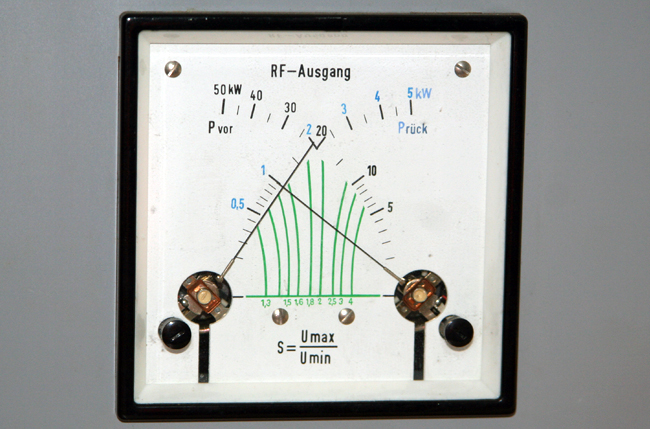
\includegraphics[width=0.85\textwidth]{foto/143}
    \caption{\scriptsize SWR-Meter mit Kreuzzeiger, linker Zeiger für die vorlaufende und rechter Zeiger für die rücklaufende Leistung; um das SWR abzulesen wird der grünen Linie am Schnittpunkt beider Zeiger nach unten gefolgt}
    \label{swr_meter_kreuzzeiger}
\end{figure}

   \end{column}
\end{columns}

\end{frame}

\begin{frame}Wird zwischen Transceiver und Antenne eingeschleift oder ist bereits im Transceiver eingebaut
\begin{columns}
    \begin{column}{0.48\textwidth}
    
\begin{figure}
    \DARCimage{0.85\linewidth}{670include}
    \caption{\scriptsize Prinzipbild SWR-Meter zwischen Transceiver  und Antenne}
    \label{n_trx_kabel_swr_antenne}
\end{figure}


    \end{column}
   \begin{column}{0.48\textwidth}
       
\begin{figure}
    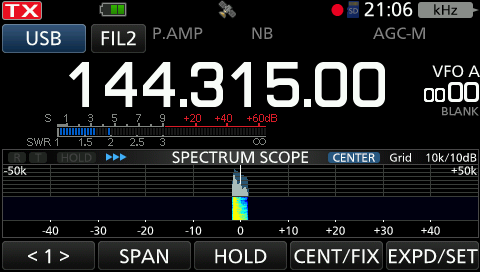
\includegraphics[width=0.85\textwidth]{foto/67}
    \caption{\scriptsize Display eines Transceivers}
    \label{n_swr_display}
\end{figure}

   \end{column}
\end{columns}

\end{frame}

\begin{frame}
\only<1>{
\begin{QQuestion}{NI201}{Mit welchem Messgerät lässt sich die Antennenanpassung bestimmen?}{Feldstärkemessgerät}
{Multimeter}
{Frequenzzähler}
{Stehwellenmessgerät}
\end{QQuestion}

}
\only<2>{
\begin{QQuestion}{NI201}{Mit welchem Messgerät lässt sich die Antennenanpassung bestimmen?}{Feldstärkemessgerät}
{Multimeter}
{Frequenzzähler}
{\textbf{\textcolor{DARCgreen}{Stehwellenmessgerät}}}
\end{QQuestion}

}
\end{frame}

\begin{frame}
\only<1>{
\begin{PQuestion}{NF101}{Die Darstellung zeigt das Display eines Transceivers im Sendebetrieb. Wie wird die Anzeige 1 bezeichnet?}{Wasserfalldiagramm}
{S-Meter}
{Amplitudenspektrum}
{SWR-Meter}
{\DARCimage{1.0\linewidth}{578include}}\end{PQuestion}

}
\only<2>{
\begin{PQuestion}{NF101}{Die Darstellung zeigt das Display eines Transceivers im Sendebetrieb. Wie wird die Anzeige 1 bezeichnet?}{Wasserfalldiagramm}
{S-Meter}
{Amplitudenspektrum}
{\textbf{\textcolor{DARCgreen}{SWR-Meter}}}
{\DARCimage{1.0\linewidth}{578include}}\end{PQuestion}

}
 \end{frame}

\begin{frame}
\only<1>{
\begin{QQuestion}{NI202}{Wenn das SWR-Meter auf der einen Seite mit der Antenne verbunden ist, was muss dann auf der anderen Seite angeschlossen werden, um Reflexionen zu messen?}{Transceiver}
{Netzteil}
{Dummy Load}
{Antennenschalter}
\end{QQuestion}

}
\only<2>{
\begin{QQuestion}{NI202}{Wenn das SWR-Meter auf der einen Seite mit der Antenne verbunden ist, was muss dann auf der anderen Seite angeschlossen werden, um Reflexionen zu messen?}{\textbf{\textcolor{DARCgreen}{Transceiver}}}
{Netzteil}
{Dummy Load}
{Antennenschalter}
\end{QQuestion}

}
\end{frame}

\begin{frame}
\frametitle{Gute Anpassung}
\begin{itemize}
  \item Bei perfekter Anpassung wird der Wert 1 angezeigt
  \item Der beste erreichbare Wert
  \end{itemize}
\end{frame}

\begin{frame}
\only<1>{
\begin{QQuestion}{NG301}{Bei welchem Stehwellenverhältnis (SWR) ist eine Antenne am besten an die Speiseleitung angepasst?}{1}
{0}
{3}
{$\mathrm{\infty}$}
\end{QQuestion}

}
\only<2>{
\begin{QQuestion}{NG301}{Bei welchem Stehwellenverhältnis (SWR) ist eine Antenne am besten an die Speiseleitung angepasst?}{\textbf{\textcolor{DARCgreen}{1}}}
{0}
{3}
{$\mathrm{\infty}$}
\end{QQuestion}

}
\end{frame}

\begin{frame}
\only<1>{
\begin{QQuestion}{NI203}{Ein Stehwellenmessgerät wird in ein ideal angepasstes Sender-/Antennensystem eingeschleift. Das Messgerät sollte~...}{ein Stehwellenverhältnis von 0 anzeigen.}
{einen Rücklauf von \qty{100}{\percent} anzeigen.}
{ein Stehwellenverhältnis von 1 anzeigen.}
{ein Stehwellenverhältnis von unendlich ($\mathrm{\infty}$) anzeigen.}
\end{QQuestion}

}
\only<2>{
\begin{QQuestion}{NI203}{Ein Stehwellenmessgerät wird in ein ideal angepasstes Sender-/Antennensystem eingeschleift. Das Messgerät sollte~...}{ein Stehwellenverhältnis von 0 anzeigen.}
{einen Rücklauf von \qty{100}{\percent} anzeigen.}
{\textbf{\textcolor{DARCgreen}{ein Stehwellenverhältnis von 1 anzeigen.}}}
{ein Stehwellenverhältnis von unendlich ($\mathrm{\infty}$) anzeigen.}
\end{QQuestion}

}
\end{frame}

\begin{frame}
\frametitle{Schlechte Anpassung}
\begin{itemize}
  \item Bei schlechter Anpassung wird nahe unendlich angezeigt
  \item Schlechte Anpassung an Übertragungsleitung
  \item Schlechte Anpassung an Antenne
  \item Defekte Übertragungsleitung
  \end{itemize}
\end{frame}

\begin{frame}
\only<1>{
\begin{PQuestion}{NG302}{Worauf deutet die dargestellte Anzeige des SWR-Meters hin?}{Eine zu hohe Sendeleistung}
{Eine gut angepasste Antenne}
{Eine schlecht angepasste Antenne}
{Eine zu geringe Sendeleistung}
{\DARCimage{1.0\linewidth}{580include}}\end{PQuestion}

}
\only<2>{
\begin{PQuestion}{NG302}{Worauf deutet die dargestellte Anzeige des SWR-Meters hin?}{Eine zu hohe Sendeleistung}
{Eine gut angepasste Antenne}
{\textbf{\textcolor{DARCgreen}{Eine schlecht angepasste Antenne}}}
{Eine zu geringe Sendeleistung}
{\DARCimage{1.0\linewidth}{580include}}\end{PQuestion}

}
\end{frame}

\begin{frame}
\only<1>{
\begin{QQuestion}{NG303}{Fehlanpassungen oder Beschädigungen von HF-Übertragungsleitungen führen~...}{zu Reflexionen des übertragenen HF-Signals und einem erhöhten SWR.}
{zu einer Überbeanspruchung der angeschlossenen Antenne.}
{zu einem SWR von kleiner oder gleich 1.}
{zur Erzeugung unerwünschter Aussendungen, da innerhalb der erforderlichen Bandbreite keine Anpassung gegeben ist.}
\end{QQuestion}

}
\only<2>{
\begin{QQuestion}{NG303}{Fehlanpassungen oder Beschädigungen von HF-Übertragungsleitungen führen~...}{\textbf{\textcolor{DARCgreen}{zu Reflexionen des übertragenen HF-Signals und einem erhöhten SWR.}}}
{zu einer Überbeanspruchung der angeschlossenen Antenne.}
{zu einem SWR von kleiner oder gleich 1.}
{zur Erzeugung unerwünschter Aussendungen, da innerhalb der erforderlichen Bandbreite keine Anpassung gegeben ist.}
\end{QQuestion}

}
\end{frame}

\begin{frame}
\frametitle{Hohe Kabeldämpfung}
\begin{itemize}
  \item Verringert das reflektierte Signal
  \item Führt zur Verfälschung der Messung
  \end{itemize}
\end{frame}

\begin{frame}
\only<1>{
\begin{QQuestion}{NG208}{Das koaxiale \qty{50}{\ohm}-Antennenkabel der \qty{2}{\m}-Amateurfunkstation wird mit einem gleichwertigen Koaxialkabel verlängert. Die Messung des SWR ergibt nach der Verlängerung einen besseren Wert. Was schließen Sie daraus? Durch die Verlängerung wird...}{die Dämpfung erhöht und das reflektierte Signal verstärkt}
{die Dämpfung verringert und das reflektierte Signal verstärkt.}
{die Dämpfung erhöht und das reflektierte Signal verringert.}
{die Dämpfung verringert und das reflektierte Signal verringert.}
\end{QQuestion}

}
\only<2>{
\begin{QQuestion}{NG208}{Das koaxiale \qty{50}{\ohm}-Antennenkabel der \qty{2}{\m}-Amateurfunkstation wird mit einem gleichwertigen Koaxialkabel verlängert. Die Messung des SWR ergibt nach der Verlängerung einen besseren Wert. Was schließen Sie daraus? Durch die Verlängerung wird...}{die Dämpfung erhöht und das reflektierte Signal verstärkt}
{die Dämpfung verringert und das reflektierte Signal verstärkt.}
{\textbf{\textcolor{DARCgreen}{die Dämpfung erhöht und das reflektierte Signal verringert.}}}
{die Dämpfung verringert und das reflektierte Signal verringert.}
\end{QQuestion}

}

\end{frame}%ENDCONTENT
